\documentclass[]{article}
\usepackage{lmodern}
\usepackage{amssymb,amsmath}
\usepackage{ifxetex,ifluatex}
\usepackage{fixltx2e} % provides \textsubscript
\ifnum 0\ifxetex 1\fi\ifluatex 1\fi=0 % if pdftex
  \usepackage[T1]{fontenc}
  \usepackage[utf8]{inputenc}
\else % if luatex or xelatex
  \ifxetex
    \usepackage{mathspec}
  \else
    \usepackage{fontspec}
  \fi
  \defaultfontfeatures{Ligatures=TeX,Scale=MatchLowercase}
\fi
% use upquote if available, for straight quotes in verbatim environments
\IfFileExists{upquote.sty}{\usepackage{upquote}}{}
% use microtype if available
\IfFileExists{microtype.sty}{%
\usepackage{microtype}
\UseMicrotypeSet[protrusion]{basicmath} % disable protrusion for tt fonts
}{}
\usepackage[margin=1in]{geometry}
\usepackage{hyperref}
\hypersetup{unicode=true,
            pdftitle={Does Chinese Classical Poems from Tang Dynasty Conform to Rhyming Rules? A Quantitative Analysis},
            pdfauthor={Lucius Hu},
            pdfborder={0 0 0},
            breaklinks=true}
\urlstyle{same}  % don't use monospace font for urls
\usepackage{color}
\usepackage{fancyvrb}
\newcommand{\VerbBar}{|}
\newcommand{\VERB}{\Verb[commandchars=\\\{\}]}
\DefineVerbatimEnvironment{Highlighting}{Verbatim}{commandchars=\\\{\}}
% Add ',fontsize=\small' for more characters per line
\usepackage{framed}
\definecolor{shadecolor}{RGB}{248,248,248}
\newenvironment{Shaded}{\begin{snugshade}}{\end{snugshade}}
\newcommand{\AlertTok}[1]{\textcolor[rgb]{0.94,0.16,0.16}{#1}}
\newcommand{\AnnotationTok}[1]{\textcolor[rgb]{0.56,0.35,0.01}{\textbf{\textit{#1}}}}
\newcommand{\AttributeTok}[1]{\textcolor[rgb]{0.77,0.63,0.00}{#1}}
\newcommand{\BaseNTok}[1]{\textcolor[rgb]{0.00,0.00,0.81}{#1}}
\newcommand{\BuiltInTok}[1]{#1}
\newcommand{\CharTok}[1]{\textcolor[rgb]{0.31,0.60,0.02}{#1}}
\newcommand{\CommentTok}[1]{\textcolor[rgb]{0.56,0.35,0.01}{\textit{#1}}}
\newcommand{\CommentVarTok}[1]{\textcolor[rgb]{0.56,0.35,0.01}{\textbf{\textit{#1}}}}
\newcommand{\ConstantTok}[1]{\textcolor[rgb]{0.00,0.00,0.00}{#1}}
\newcommand{\ControlFlowTok}[1]{\textcolor[rgb]{0.13,0.29,0.53}{\textbf{#1}}}
\newcommand{\DataTypeTok}[1]{\textcolor[rgb]{0.13,0.29,0.53}{#1}}
\newcommand{\DecValTok}[1]{\textcolor[rgb]{0.00,0.00,0.81}{#1}}
\newcommand{\DocumentationTok}[1]{\textcolor[rgb]{0.56,0.35,0.01}{\textbf{\textit{#1}}}}
\newcommand{\ErrorTok}[1]{\textcolor[rgb]{0.64,0.00,0.00}{\textbf{#1}}}
\newcommand{\ExtensionTok}[1]{#1}
\newcommand{\FloatTok}[1]{\textcolor[rgb]{0.00,0.00,0.81}{#1}}
\newcommand{\FunctionTok}[1]{\textcolor[rgb]{0.00,0.00,0.00}{#1}}
\newcommand{\ImportTok}[1]{#1}
\newcommand{\InformationTok}[1]{\textcolor[rgb]{0.56,0.35,0.01}{\textbf{\textit{#1}}}}
\newcommand{\KeywordTok}[1]{\textcolor[rgb]{0.13,0.29,0.53}{\textbf{#1}}}
\newcommand{\NormalTok}[1]{#1}
\newcommand{\OperatorTok}[1]{\textcolor[rgb]{0.81,0.36,0.00}{\textbf{#1}}}
\newcommand{\OtherTok}[1]{\textcolor[rgb]{0.56,0.35,0.01}{#1}}
\newcommand{\PreprocessorTok}[1]{\textcolor[rgb]{0.56,0.35,0.01}{\textit{#1}}}
\newcommand{\RegionMarkerTok}[1]{#1}
\newcommand{\SpecialCharTok}[1]{\textcolor[rgb]{0.00,0.00,0.00}{#1}}
\newcommand{\SpecialStringTok}[1]{\textcolor[rgb]{0.31,0.60,0.02}{#1}}
\newcommand{\StringTok}[1]{\textcolor[rgb]{0.31,0.60,0.02}{#1}}
\newcommand{\VariableTok}[1]{\textcolor[rgb]{0.00,0.00,0.00}{#1}}
\newcommand{\VerbatimStringTok}[1]{\textcolor[rgb]{0.31,0.60,0.02}{#1}}
\newcommand{\WarningTok}[1]{\textcolor[rgb]{0.56,0.35,0.01}{\textbf{\textit{#1}}}}
\usepackage{graphicx,grffile}
\makeatletter
\def\maxwidth{\ifdim\Gin@nat@width>\linewidth\linewidth\else\Gin@nat@width\fi}
\def\maxheight{\ifdim\Gin@nat@height>\textheight\textheight\else\Gin@nat@height\fi}
\makeatother
% Scale images if necessary, so that they will not overflow the page
% margins by default, and it is still possible to overwrite the defaults
% using explicit options in \includegraphics[width, height, ...]{}
\setkeys{Gin}{width=\maxwidth,height=\maxheight,keepaspectratio}
\IfFileExists{parskip.sty}{%
\usepackage{parskip}
}{% else
\setlength{\parindent}{0pt}
\setlength{\parskip}{6pt plus 2pt minus 1pt}
}
\setlength{\emergencystretch}{3em}  % prevent overfull lines
\providecommand{\tightlist}{%
  \setlength{\itemsep}{0pt}\setlength{\parskip}{0pt}}
\setcounter{secnumdepth}{0}
% Redefines (sub)paragraphs to behave more like sections
\ifx\paragraph\undefined\else
\let\oldparagraph\paragraph
\renewcommand{\paragraph}[1]{\oldparagraph{#1}\mbox{}}
\fi
\ifx\subparagraph\undefined\else
\let\oldsubparagraph\subparagraph
\renewcommand{\subparagraph}[1]{\oldsubparagraph{#1}\mbox{}}
\fi

%%% Use protect on footnotes to avoid problems with footnotes in titles
\let\rmarkdownfootnote\footnote%
\def\footnote{\protect\rmarkdownfootnote}

%%% Change title format to be more compact
\usepackage{titling}

% Create subtitle command for use in maketitle
\providecommand{\subtitle}[1]{
  \posttitle{
    \begin{center}\large#1\end{center}
    }
}

\setlength{\droptitle}{-2em}

  \title{Does Chinese Classical Poems from Tang Dynasty Conform to Rhyming Rules?
A Quantitative Analysis}
    \pretitle{\vspace{\droptitle}\centering\huge}
  \posttitle{\par}
    \author{Lucius Hu}
    \preauthor{\centering\large\emph}
  \postauthor{\par}
      \predate{\centering\large\emph}
  \postdate{\par}
    \date{May 9, 2019}

\usepackage{ctex}
\setCJKmainfont{Sarasa Gothic CL}

\begin{document}
\maketitle

\hypertarget{intorduction}{%
\subsection{Intorduction}\label{intorduction}}

In Tang Dynasty of China, there emerged two types of rhyming poems,
\emph{LüShi} and \emph{JueJu}, whose literal translations are
\emph{regulated verse} and \emph{cut-off lines} respectively. The former
one must have 8 sentences while the latter one shall have 4 sentences.
Each sentence of either LüShi or JueJu shall have a fixed number of
characters, either 5 or 7. Hence, those Tang poems are categorised into
the followings according to the number of lines and the number of
characters in each line:

\begin{itemize}
\tightlist
\item
  WuLü: 5-character 8-line regular verse
\item
  QiLü: 7-character 8-line regular verse
\item
  WuJue: 5-character quatrain
\item
  QiJue: 7-character quatrain
\end{itemize}

Phoenetically, there is a complex set of rules regulating what
characters could be allowed to be put into a certain position.
Specifically, LüShi requires the last character of the 2nd, 4th, 6th,
and 8th lines to be rhyming characters, and meanwhile JueJu requires
last characters from the 2nd and 4th lines to rhyme with each other.

When writing a peom, its author not only needs to conform to the
phoenetical rules, but also need to pay attention to the wording, and
more importantly, exhibit its aethetical value. Thus it would take many
years for a person to write a qualified poem, and only a very small
number of poems ever written were good enough to be passed on through
generations.

There's a collection of Tang Poems, \emph{Three Hundred Tang Poems},
that contains 317 poems from Tang Dynasty. Among them, there are 227
poems that belong to the four aforementioned categories. It is
interesting to know to what extent does these poems conform to the
rhyming rules.

Specifically, there might be two types of reason that a poet would
violate the rules. First, the author speaks a different variety of
Chinese which experience some phoenetical change from the `official
language' during Tang Dynasty. Second, it's just very hard to find a
rhyming characters and the author chose to sacrifice the phoenetics for
better literature, and/or philosophical value.

\hypertarget{acquiring-the-text-corpus-of-three-hundred-tang-poems}{%
\subsection{Acquiring the Text Corpus of Three Hundred Tang
Poems}\label{acquiring-the-text-corpus-of-three-hundred-tang-poems}}

The first data source is Wikisource, which has the full text body of
Three Hundred Tang Poems. The table of contents of Three Hundred Tang
Poems is available
\href{'https://zh.wikisource.org/wiki/唐詩三百首'}{here}. We will first
extract the links to the four aforementioned categories of poems, and
then download the html pages given the URLs. Then we will extract the
text body from html source code using `rvest' package.

\begin{Shaded}
\begin{Highlighting}[]
\KeywordTok{source}\NormalTok{(}\StringTok{'initialisation.R'}\NormalTok{)}
\NormalTok{DT <-}\StringTok{ }\KeywordTok{dlMenu}\NormalTok{()}
\KeywordTok{str}\NormalTok{(DT[}\DecValTok{1}\NormalTok{])}
\end{Highlighting}
\end{Shaded}

\begin{verbatim}
## Classes 'data.table' and 'data.frame':   1 obs. of  4 variables:
##  $ type  : chr "Wulü"
##  $ author: chr "王勃"
##  $ title : chr "送杜少府之任蜀州"
##  $ url   : chr "https://zh.wikisource.org/wiki/%E9%80%81%E6%9D%9C%E5%B0%91%E5%BA%9C%E4%B9%8B%E4%BB%BB%E8%9C%80%E5%B7%9E"
##  - attr(*, ".internal.selfref")=<externalptr>
\end{verbatim}

Most Wikisource pages we encountered has similar structures and most
links to the poems are correct, thus there's not much difficulty for the
text extraction. Specifically, each peom is in a '

`node, which has 4 child nodes with'

' tags (paragraph), which contains two sentences of LüShi or one
sentence of JueJu.

Next, we just need to remove all empty lines and punctuations in the end
of each sentences, which are one of the followings:

\begin{itemize}
\tightlist
\item
  `~' (Halfwidth) Whitespace Character
\item
  ` ' Fullwidth White Space Character
\item
  `,' Fullwidth Comma
\item
  `。' Fullwidth Period
\item
  `?' Fullwidth Question Mark
\item
  `!' Fullwidth Exclamation Mark
\item
  `;' Fullwidth Semicolon
\end{itemize}

In a small number of poems, there also contains footnotes, which takes
one of the two following forms:

\begin{itemize}
\tightlist
\item
  `〈\ldots{}〉' Footnotes between Fullwidth Opening Left-Angle Bracket
  and Fullwidth Right-Angle Bracket
\item
  `{[}\ldots{}{]}' Fottnotes between (Halfwidth) Left Bracket and
  (Halfwidth) Right Bracket
\end{itemize}

Below is a excerpt of codes we used to obtain the the text corpus.

\begin{Shaded}
\begin{Highlighting}[]
\NormalTok{newtext <-}
\StringTok{      }\KeywordTok{read_html}\NormalTok{(f, }\DataTypeTok{encoding =} \StringTok{'UTF-8'}\NormalTok{) }\OperatorTok
\StringTok{      }\KeywordTok{html_nodes}\NormalTok{(}\StringTok{'div.poem p'}\NormalTok{) }\OperatorTok
\StringTok{      }\KeywordTok{html_text}\NormalTok{() }\OperatorTok
\StringTok{      }\CommentTok{# must first remove new-line character so the other regex}
\StringTok{      }\CommentTok{# would be correctly applied to multi-lines}
\StringTok{      }\KeywordTok{str_remove_all}\NormalTok{(}\StringTok{'}\CharTok{\textbackslash{}\textbackslash{}}\StringTok{n'}\NormalTok{) }\OperatorTok
\StringTok{      }\KeywordTok{str_remove_all}\NormalTok{(}\StringTok{'〈.+?〉|}\CharTok{\textbackslash{}\textbackslash{}}\StringTok{[.+?}\CharTok{\textbackslash{}\textbackslash{}}\StringTok{]| | |,|。|?|!|;'}\NormalTok{)}
\NormalTok{text <-}\StringTok{ }\KeywordTok{c}\NormalTok{(text, newtext)}
\end{Highlighting}
\end{Shaded}

But instead of analysing the full text corpus, actually we need only the
last characters of the even-numbered sentences. First, depends on the
category to which a poem belong, the index of the characters we need to
keep is different. The following lines show the way how we defined the
four possible cases, with the `switch' control flow:

\begin{Shaded}
\begin{Highlighting}[]
\NormalTok{idx <-}\StringTok{ }\ControlFlowTok{function}\NormalTok{(type) \{}
    \ControlFlowTok{switch}\NormalTok{(type,}
\NormalTok{           Wulü  =}\StringTok{ }\KeywordTok{seq}\NormalTok{(}\DecValTok{10}\NormalTok{, }\DecValTok{40}\NormalTok{, }\DecValTok{10}\NormalTok{),}
\NormalTok{           Qilü  =}\StringTok{ }\KeywordTok{seq}\NormalTok{(}\DecValTok{14}\NormalTok{, }\DecValTok{56}\NormalTok{, }\DecValTok{14}\NormalTok{),}
           \DataTypeTok{Wujue =} \KeywordTok{seq}\NormalTok{(}\DecValTok{10}\NormalTok{, }\DecValTok{20}\NormalTok{, }\DecValTok{10}\NormalTok{),}
           \DataTypeTok{Qijue =} \KeywordTok{seq}\NormalTok{(}\DecValTok{14}\NormalTok{, }\DecValTok{28}\NormalTok{, }\DecValTok{14}\NormalTok{))}
\NormalTok{  \}}
\end{Highlighting}
\end{Shaded}

Then, with the aide of `purrr' package, we wrote a `mapper' and apply
each poems to it:

\begin{Shaded}
\begin{Highlighting}[]
\KeywordTok{pmap}\NormalTok{(data[,.(type, text)],}
       \ControlFlowTok{function}\NormalTok{(type, text) \{}
\NormalTok{         nextChar <-}\StringTok{ }\KeywordTok{character}\NormalTok{()}
         \ControlFlowTok{for}\NormalTok{ (i }\ControlFlowTok{in} \KeywordTok{idx}\NormalTok{(type)) \{}
\NormalTok{           nextChar <-}\StringTok{ }\KeywordTok{c}\NormalTok{(nextChar, }\KeywordTok{str_sub}\NormalTok{(text, i, i))}
\NormalTok{         \}}
\NormalTok{         nextChar <-}\StringTok{ }\KeywordTok{paste0}\NormalTok{(nextChar, }\DataTypeTok{collapse =} \StringTok{''}\NormalTok{)}
\NormalTok{       \}}
\NormalTok{  )}
\end{Highlighting}
\end{Shaded}

Below shows how the data table look like, which contains the meta-data,
i.e.~type, author, title, as well as the urls, and both the full text
and last characters we just extracted.

\begin{Shaded}
\begin{Highlighting}[]
\KeywordTok{source}\NormalTok{(}\StringTok{'processPoems.R'}\NormalTok{)}
\KeywordTok{str}\NormalTok{(DT[}\DecValTok{1}\NormalTok{])}
\end{Highlighting}
\end{Shaded}

\begin{verbatim}
## Classes 'data.table' and 'data.frame':   1 obs. of  6 variables:
##  $ type    : chr "Wulü"
##  $ author  : chr "王勃"
##  $ title   : chr "送杜少府之任蜀州"
##  $ url     : chr "https://zh.wikisource.org/wiki/%E9%80%81%E6%9D%9C%E5%B0%91%E5%BA%9C%E4%B9%8B%E4%BB%BB%E8%9C%80%E5%B7%9E"
##  $ text    : chr "城闕輔三秦風煙望五津與君離別意同是宦遊人海內存知己天涯若比隣無爲在岐路兒女共霑巾"
##  $ lastChar:List of 1
##   ..$ : chr "津人隣巾"
##  - attr(*, ".internal.selfref")=<externalptr>
\end{verbatim}

\hypertarget{acquiring-the-rhymes-of-the-last-characters-we-extracted}{%
\subsection{Acquiring the Rhymes of the Last Characters we
extracted}\label{acquiring-the-rhymes-of-the-last-characters-we-extracted}}

At this point, we already get the set of characters, and we will need to
get their rhymes. But first we will give a brief introduction to the
second data source, from which we would obtained the rhymes.

\url{https://ytenx.org} is a website which allows the users to query
phonetic attributes of a Chinese character, including the consonant,
vowels, tones, definitions, and rhymes. Notice that rhymes and vowels
are two related but distinct concept. If two characters have same
vowels, they must rhyme with each other. But rhyming characters may have
similar rather than identical vowels.

In Chinese Linguistic studies, the official language across the history
are, \emph{Old Chinese}, \emph{Middle Chinese}, \emph{Old Mandarin}, and
\emph{Mordern Mandarin}, in chronological order. The Old Mandarin and
Modern Mandarin are both Mandarin language. But neither Old Chinese nor
Middle Chinese is refering to \emph{a} language, but rather \emph{a
family} of Chinese Languages.

The information available at \url{https://ytenx.org} are provided by
volunteers, based on the authetic phoenetic dictionaries such as
\emph{上古音系}, \emph{廣韻},\emph{洪武正韻牋}, \emph{中原音韻}, and
\emph{分韻撮要}, which corresponds to Old Chinese, Middle Chinese,
Sourthern Old Mandarin, Northern Old Mandarin, and Old Cantonese,
respectively. During Tang Dynasty, the official language was Middle
Chinese, and thus we need to get the data from 廣韻.

The following shows how the rhymes are extracted. First, similar to the
extraction of text body, we initiate a HTML request and read the HTML
source code of the response, and we use the html tag `p yohn' and `href'
to find the link to the details page of a given character. On the detail
page there's a HTML table, and there's a row named `韻攝', which contain
the rhyme of the given character. And we will assign `X' if the queried
character is not found.

\begin{Shaded}
\begin{Highlighting}[]
\NormalTok{rhm <-}
\StringTok{      }\KeywordTok{glue}\NormalTok{(}
        \StringTok{'http://ytenx.org/zim?dzih=\{c\}&kyonh=1&jtkb=1&jtdt=1&jtkd=1&jtgt=1'}
\NormalTok{      ) }\OperatorTok
\StringTok{      }\KeywordTok{read_html}\NormalTok{() }\OperatorTok
\StringTok{      }\KeywordTok{html_node}\NormalTok{(}\StringTok{'p.yonh a'}\NormalTok{) }\OperatorTok
\StringTok{      }\KeywordTok{html_attr}\NormalTok{(}\StringTok{'href'}\NormalTok{)}
    \ControlFlowTok{if}\NormalTok{ (}\OperatorTok{!}\KeywordTok{is.na}\NormalTok{(rhm)) \{}
\NormalTok{      rhm <-}
\StringTok{        }\KeywordTok{glue}\NormalTok{(}\StringTok{'http://ytenx.org\{rhm\}'}\NormalTok{) }\OperatorTok
\StringTok{        }\KeywordTok{read_html}\NormalTok{() }\OperatorTok
\StringTok{        }\KeywordTok{html_table}\NormalTok{() }\OperatorTok\StringTok{ }\NormalTok{.[[}\DecValTok{1}\NormalTok{]]}
\NormalTok{      rhm <-}
\StringTok{        }\NormalTok{rhm[}\KeywordTok{which}\NormalTok{(rhm}\OperatorTok{$}\StringTok{'X1'} \OperatorTok{==}\StringTok{ '韻攝'}\NormalTok{),}\DecValTok{2}\NormalTok{]}
\NormalTok{    \} }\ControlFlowTok{else}\NormalTok{ \{}
\NormalTok{      rhm <-}\StringTok{ 'X'}
\NormalTok{    \}}
\end{Highlighting}
\end{Shaded}

Based on the rhymes we extracted, we now have a data frame where the
first column is a character, and the second column is its rhyme. This
data frame would serve us as a look-up table, and we will write a mapper
to match each character to a rhyme according to the look-up table.

\begin{Shaded}
\begin{Highlighting}[]
\KeywordTok{map}\NormalTok{(data,}
      \ControlFlowTok{function}\NormalTok{(x) \{}
\NormalTok{        nextRhyme <-}\StringTok{ }\KeywordTok{character}\NormalTok{()}
        \ControlFlowTok{for}\NormalTok{ (i }\ControlFlowTok{in} \KeywordTok{unlist}\NormalTok{(}\KeywordTok{str_split}\NormalTok{(x, }\StringTok{''}\NormalTok{))) \{}
\NormalTok{          nextRhyme <-}\StringTok{ }\KeywordTok{c}\NormalTok{(nextRhyme, dict[char }\OperatorTok{==}\StringTok{ }\NormalTok{i]}\OperatorTok{$}\NormalTok{rhymes)}
\NormalTok{        \}}
\NormalTok{        nextRhyme <-}\StringTok{ }\KeywordTok{paste0}\NormalTok{(nextRhyme, }\DataTypeTok{collapse =} \StringTok{''}\NormalTok{)}
\NormalTok{      \})}
\end{Highlighting}
\end{Shaded}

Here is an example of the matched characters and their rhymes for the
first five lines of our data, where each line corresponds to a poem.

\begin{Shaded}
\begin{Highlighting}[]
\KeywordTok{source}\NormalTok{(}\StringTok{'processRhymes.R'}\NormalTok{)}
\KeywordTok{head}\NormalTok{(DT[, .(lastChar, rhymes)], }\DecValTok{5}\NormalTok{)}
\end{Highlighting}
\end{Shaded}

\begin{verbatim}
##    lastChar      rhymes
## 1: 津人隣巾 臻 臻 臻 臻
## 2: 鵑泉田賢 山 山 山 山
## 3: 通中空翁 通 通 通 通
## 4: 陲知時期 止 止 止 止
## 5: 隅無殊夫 遇 遇 遇 遇
\end{verbatim}

\hypertarget{exploratary-analysis}{%
\section{Exploratary Analysis}\label{exploratary-analysis}}

First, let's check the proportion of poems in each of the four
categories that strictly conform to the rhyming rules. Based on the
rhymes, we also appended a new columns of boolean variable, indicating
whether the the rhyming characters are all having one identical rhyme.

As we can see, it indeed seems easier to follow the rules when you only
need to write four lines, as in Jueju, as oppose to LüShi, when you need
to write eight lines. Secondly, for both LüShi and JueJu, it's easier to
follow the rule when you the number of character is fewer.

\begin{Shaded}
\begin{Highlighting}[]
\NormalTok{DT[, .(}\DataTypeTok{proportion =} \KeywordTok{sum}\NormalTok{(.SD}\OperatorTok{$}\NormalTok{correctRhyming)}\OperatorTok{/}\KeywordTok{nrow}\NormalTok{(.SD)), by =}\StringTok{ }\NormalTok{type]}
\end{Highlighting}
\end{Shaded}

\begin{verbatim}
##     type proportion
## 1:  Wulü  0.8750000
## 2:  Qilü  0.8490566
## 3: Wujue  1.0000000
## 4: Qijue  0.9215686
\end{verbatim}

And if we plot such proportion against the number of character, than we
will have the following visualisation. And obviously, there is a
negative correlation between the total number of characters in a poem,
and the tendency that it would strictly conform to the rhyming rules.
This coincides with our gut sense that more characters imposes a greater
difficulty on rhyming.

\begin{Shaded}
\begin{Highlighting}[]
\NormalTok{p <-}\StringTok{ }\KeywordTok{paste0}\NormalTok{(}\KeywordTok{tempfile}\NormalTok{(),}\StringTok{'.png'}\NormalTok{) }
\KeywordTok{ggsave}\NormalTok{(p,}
       \KeywordTok{ggplot}\NormalTok{(}
\NormalTok{         DT[ ,}
\NormalTok{             .(}\DataTypeTok{proportion =} \KeywordTok{sum}\NormalTok{(.SD}\OperatorTok{$}\NormalTok{correctRhyming)}\OperatorTok{/}\KeywordTok{nrow}\NormalTok{(.SD)),}
             \DataTypeTok{by =}\NormalTok{ type][ ,}
                         \StringTok{'#ofCharacters'} \OperatorTok{:}\ErrorTok{=}\StringTok{ }\KeywordTok{c}\NormalTok{(}\DecValTok{40}\NormalTok{, }\DecValTok{56}\NormalTok{, }\DecValTok{20}\NormalTok{, }\DecValTok{28}\NormalTok{)]) }\OperatorTok{+}
\StringTok{    }\KeywordTok{geom_line}\NormalTok{(}\KeywordTok{aes}\NormalTok{(}\DataTypeTok{y =}\NormalTok{ proportion, }\DataTypeTok{x =} \StringTok{`}\DataTypeTok{#ofCharacters}\StringTok{`}\NormalTok{)))}
\KeywordTok{grid.raster}\NormalTok{(}\KeywordTok{readPNG}\NormalTok{(p,}\StringTok{'.png'}\NormalTok{))}
\end{Highlighting}
\end{Shaded}

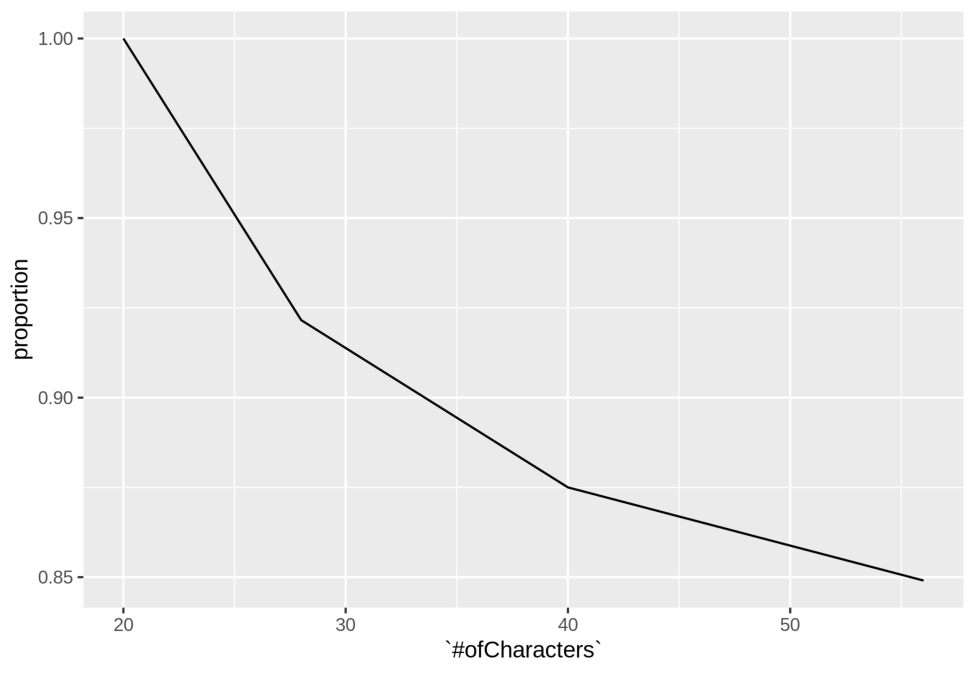
\includegraphics{main_files/figure-latex/unnamed-chunk-11-1.pdf}

Last, we may also check the what rhymes are more often used.

\begin{Shaded}
\begin{Highlighting}[]
\NormalTok{p <-}\StringTok{ }\KeywordTok{paste0}\NormalTok{(}\KeywordTok{tempfile}\NormalTok{(),}\StringTok{'.png'}\NormalTok{) }
\KeywordTok{ggsave}\NormalTok{(p, }\DataTypeTok{plot =} \KeywordTok{ggplot}\NormalTok{(DTRhymes) }\OperatorTok{+}\StringTok{ }\KeywordTok{geom_histogram}\NormalTok{(}\KeywordTok{aes}\NormalTok{(rhymes), }\DataTypeTok{stat =} \StringTok{'count'}\NormalTok{))}
\KeywordTok{grid.raster}\NormalTok{(}\KeywordTok{readPNG}\NormalTok{(p,}\StringTok{'.png'}\NormalTok{))}
\end{Highlighting}
\end{Shaded}

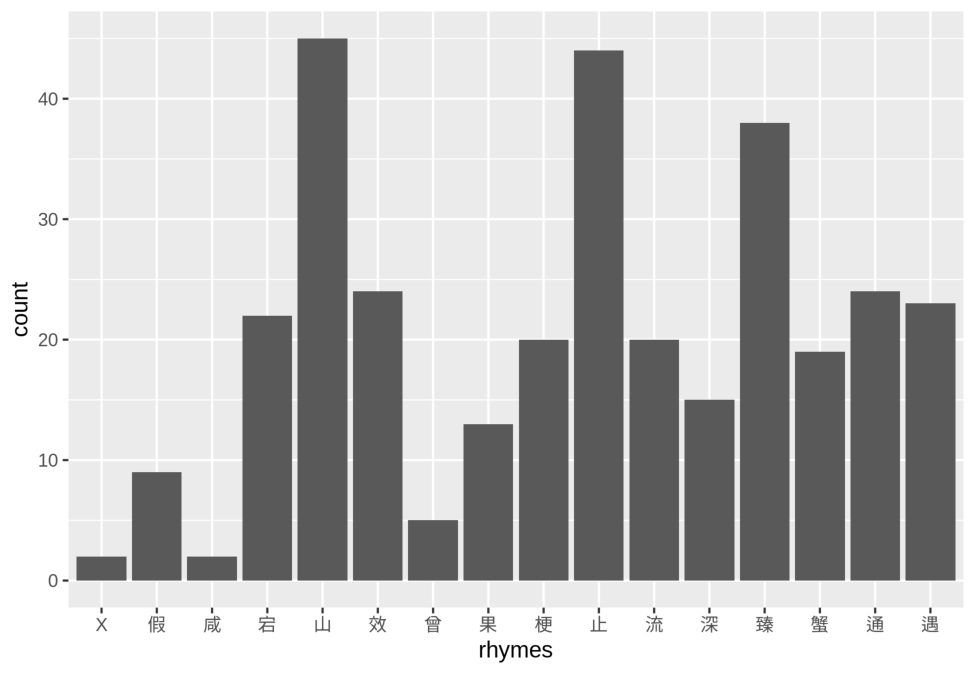
\includegraphics{main_files/figure-latex/unnamed-chunk-12-1.pdf}


\end{document}
